\documentclass[twocolumn]{article}
\usepackage{titling,float,titlesec,tikz,amsmath,amssymb,pdfpages,graphicx,array}
\usepackage[dvipsnames]{xcolor}
\newcommand{\note}[1] {
	\textcolor{Purple}{#1}

}

\title{Practical Runtime Verification of Performance in event based systems using Metric Temporal Logic}

\author{George Fakidis}

\begin{document}
\maketitle
\begin{abstract}
	Event Based Systems(EBS) are the foundation of modern cloud system infrastructure. Event Driven Architecture(EDA) is a scalable architectural pattern that enables operations at an unprecedented scale. Performance considerations are of utmost importance to ensure cost efficiency and achieving QoS guarantees.
	In this paper we demonstrate a formal approach of performance monitoring in an EBS, in a manner that allows us to reuse existing methodologies and algorithms, using a combination of Metric Temporal Logic(MTL) and EBS formalisations.
	We show that performance monitoring of a series of events can be solved by checking the temporal constraints of the events under study using metric temporal logic.
	We also design a preliminary tool to integrate this runtime verification into existing technology stacks, which will be demonstrated in future work.
\end{abstract}


\section{Introduction}

Software Systems have grown considerably in the last years, and are now used in critical sectors like 1,2,3.
Modern large scale systems serve millions of users and execute billions of operations per second.
To enable computation at this unprecedented scale, sophisticated scalable architectures are required.
One of the most popular and widely adopted is Event-Driven Architecture(EDA) that centers its attention to messages sent between different systems in order to complete the desired computations.
Therefore it is necessary to reason about the performance and correctness software and systems in a manner that can provide guarantees and be relied upon. Event-based systems are complex due to the flexible,unspecified and asynchronous interactions they enable and thus require expressive specification techniques that can be checked at runtime.
\par
Formal Methods are a set of mathematical tools that enable us to reason about software in a complete, sound and verifiable manner using specifications that can be checked rigorously. Runtime verification uses data generated by a running system(event logs,traces) in order to detect violations of expressed properties and tries to provide guarantees for the system being studied.



\section{Metric Temporal Logic}
In this section we give a brief and practical explanation of Metric Temporal Logic, for a more mathematically rigorous presentation of the concepts presented here the reader is referred to \cite{hendriks_checking_2016,dhananjayan_metric_2014,thati_monitoring_2005,pnueli_temporal_1977}.
\par
Linear Temporal Logic(LTL) \cite{pnueli_temporal_1977} allows us to reason about propositions' truth values across a linear timeline.
MTL \cite{koymans_specifying_1990} is an extension of LTL that enhances temporal operators with timing constraints. The temporal operators are (U)ntil, (R)elease, (N)ext, (F)uture, (G)lobally, (A)lways, (E)xists.
This enables us to reason about performance in a concise and mathematically rigorous manner, taking advantage of existing
monitoring algorithms for MTL specifications.

\par
To understand MTL, we start with a finite set of propositional variables, denoted by $AP$.
At each point in time there is a state $S$, that carries the truth values of all $AP$ propositions.
MTL formulas are then checked against a timed \emph{trace}, where trace is a (possibly infinte) sequence of states in $S$.
A \emph{timed trace} is a sequence of tuple elements in $S \times T$, where $T$ is a monotonically increasing sequence of timestamps.
We can then evaluate MTL specifications on timed traces.
MTL provides us a way to concisely specify performance expectations of the system being monitored, in a generic and expressive manner.

\par
The syntax of MTL can be defined as follows:
\[
	\varphi \; := \; true \; | \; p \; | \; \varphi \land \varphi \; | \; \varphi \lor \varphi \;| \; \neg \varphi \; | \; \varphi \mathcal{U}_I \varphi \quad p \in \mathbf{AP}
\]

$U_I$ denotes the \emph{Until} temporal operator in interval \emph{I}, from which the rest of the operators are derived from.
The remaining operators mentioned previously can be seen in Table~\ref{table:mtl_operators}, which will
be further showcased in practical examples.

\begin{table*}[h]
	\small\centering
	\renewcommand{\arraystretch}{1.5}
	\begin{tabular}{|c|c|l|}
		\hline
		\textbf{Operator}    & \textbf{Symbol}              & \textbf{Meaning}                                                            \\
		\hline
		Until                & $\varphi \mathcal{U}_I \psi$ & $\varphi$ holds until $\psi$ becomes true within interval $I$.              \\
		\hline
		Release              & $\varphi \mathcal{R}_I \psi$ & $\psi$ remains true until the first time $\varphi$ becomes true within $I$. \\
		\hline
		Next                 & $\bigcirc_I \varphi$         & $\varphi$ holds at the next time step within $I$.                           \\
		\hline
		Finally (Eventually) & $\Diamond_I \varphi$         & $\varphi$ will eventually hold at some time within $I$.                     \\
		\hline
		Globally (Always)    & $\Box_I \varphi$             & $\varphi$ must hold at all time points within $I$.                          \\
		\hline
	\end{tabular}
	\caption{Temporal Operators in Metric Temporal Logic (MTL)}
	\label{table:mtl_operators}
\end{table*}


\section{Related Work}

In \cite{trinh_checking_2024}, the authors present a formalisation of EBS systems based on Allen's \cite{allen_maintaining_1983} temporal interval relations and provide a checking algorithm for the model.
In \cite{ganguly_distributed_2024}, the authors demonstrate a way to utilise MTL in a partially synchronous distributed system where there is not a single global clock. They also provide a way to evaluate MTL expressions incrementally by rewriting the formulas.
In \cite{mackey_early_2024}, the authors provide a formalisation and the respective algorithms using an approach based on workflows and events to proactively detect timing constraints violations in rules.

In \cite{hendriks_checking_2016}, the authors introduce a novel tool to check metric temporal logic formulas. The online runtime verification scenario is not fully handled in the tool.
The conceptual framework supports it through the use of "informative prefixes", a construct that defines how partial traces can be used to inform us about the truth value of a formula $\varphi$.
In \cite{dhananjayan_metric_2014}, the authors demonstrate how MTL can be used as an expressive and readable intermediate specification for timed transition graphs in the context of timed discrete-event systems.

In \cite{paterson_observation-enhanced_2018}, the authors present a method for checking QoS properties, using a continuous-time Markov Chain(CTMC), in the context of component based systems. They also present an automated tool, and two case studies, one of which is based on a service-based system.

In \cite{mammar_formal_2024}, the authors use the Event-B formal method for modelling and analysis in the deployment of cloud applications.

In \cite{xavier_framework_2024}, the authors generate a model and a monitor of an industrial system ({IEC 61499 Standard}) using process mining from event logs in order to formally verify event-driven systems.


\section{Formalising Event-Based Systems}
We borrow formalisations for Workflows,"Enactments",Activities and Events from the work of \cite{mackey_early_2024}. Briefly explained, Workflows are an abstract series of abstract events/activities, that have a {\it start} event and possibly multiple {\it end} events.
\emph{Activities} are the lowest level building block, denoting a unit of work in workflow.
\emph{Events} are generated by the execution of an activity.
\emph{Enactments} are the result of a concrete execution of workflow. In order to be able to distinguish between different executions of the same workflow, enactments also include an ID.
This ID is included in events generated by activities execution in an enactment. In practice, this ID could be a user's ID that is carried throughout the workflow, thus allowing us to specify and monitor performance properties for the specific sequence of events while the model remains abstract and generic.

\par
Using the definitions explained above, performance in this paper is regarded as the distance between event timestamps
in order to keep the model simple.
In future work, that difference between event timestamps could be analysed in a more granular level,for example dividing the time required for responding to an event into network latency, database latency and processing latency.

\section{Formal properties in MTL}

\note{From the non my work stuff this will come first as it is important}
Metric Temporal Logic can be used as a specification language to specify desired properties of an event-based system.
When attempting to specify formal properties in a non-trivial software system it is important to understand {\it Safety} and {\it Liveness} properties \cite{lamport_what_1983} , a distinction practically and conceptually useful.
Safety is about checking whether {\it bad things} happen, it is about prohibiting invalid behaviour, thus only allowing for safe states throughout execution.

Liveness is about checking {\it good things} that must happen during an execution. It is important to note that the thing we check can involve an infinite number of steps.

Generally it is more difficult to specify and check liveness properties than safety properties[citation needed].


In the context of an event-based system we provide some indicative properties we would want to check. In Table~\ref{table:mtl_formulas} we specify the following properties to be checked. In future work, those could be expanded upon by investigating alerting and monitoring techniques and practices along with testing methodologies for EDA systems.
\begin{itemize}
	\item Event A should always be followed by Event B within a certain time(response time).
	\item Event A should be responded with Event B or Event C within a certain time(useful to specify where failures can happen and how).
	\item Event chains, e.g. Event A should be followed by Event B which should then be followed by Event C or Event D. This is especially useful when checking that execution of workflows, as defined above, conform to performance standards.
	\item Event A and Event B should not happen until another event C happens.
\end{itemize}
In a practical scenario, the above properties will represent policy that must be adhered to by the implemented software, and responses to violations shall be specified in more detail.


\begin{table*}[t]
	\centering
	\renewcommand{\arraystretch}{1.5}
	\begin{tabular}{|p{10cm}|c|}
		\hline
		\textbf{Description}                                                                                           & \textbf{MTL Formula} \\
		\hline
		Event A should always be followed by Event B within a certain time \( t \):                                    &
		$\Box (A \implies \lozenge_{\leq t} B)$                                                                                               \\
		\hline
		Event A should be responded with Event B or Event C within a certain time \( t \):                             &
		$\Box (A \implies \lozenge_{\leq t} (B \lor C))$                                                                                      \\
		\hline
		Event chains, e.g., Event A should be followed by Event B which should then be followed by Event C or Event D: &
		$\Box (A \implies \lozenge_{\leq t_1} (B \land \lozenge_{\leq t_2} (C \lor D)))$                                                      \\
		\hline
		Event A and Event B should not happen until another event happens:                                             &
		$\Box (\neg (A \lor B) \mathcal{U_I} C)$                                                                                              \\
		\hline
	\end{tabular}
	\caption{Metric Temporal Logic (MTL) Formulas for Event Constraints}
	\label{table:mtl_formulas}
\end{table*}


\section{Software Solution Design}
In this section we will talk more in detail about how to implement runtime verification of performance using metric temporal logic.

\subsection{Design Goals}
The target software architecture we intend to verify is Event-Driven Architecture(EDA), therefore any stated desired goal
should consider the constraints of a distributed event-driven architecture.

We outline the following Design Goals and explain them more in detail.

\begin{itemize}
	\item Online execution for real-time violation reports.
	\item Integration with the existing event-driven ecosystem.(Ease of Integration with a new system)
	\item Horizontal Scalability and Distributed Computation
	\item System Independent
	\item Performance
\end{itemize}


\par
\emph{Online execution} is important as the order of magnitude of the data an offline algorithm would need to store is impractical.
It also provides valuable timely feedback, useful for addressing performance issues early on and avoiding costly downtimes.
Finally the runtime verification problem by its very nature is more accurately expressed by online algorithms, an offline mode
would not differ significantly from a simple constraint checking problem using the system logs. In this paper, we focus on the online case.
\par
Being \emph{system independent} practically means that the solution does not have a model of the underlying system, only a generic view of it.
Decoupling from a concrete implementation is necessary, due to the fact that in EDA, the only common denominator between different systems
is the Event Bus, which is also further segmented into different independent topics. Assuming a specific technology stack is an approach that
is unrealistic for complex large-scale systems.
\par
\emph{Performance} is important to the degree that existing systems are not affected by the addition of the monitoring component into the system.
As with all performance measurement tools its resource consumption should be a negligible fraction of the total resource consumption of the system.
Data structures and algorithms should be carefully considered to achieve low time and space complexity. Such large-scale systems operate on the order
of magnitude of billion operations processed per second thus complexity is crucial in practice.
\par
For verification to be practical it should be close to the software development process and not implemented in a separate isolated tool.
Instead, a solution should be part of the suite of tools that is already used in EDA systems. This way not only the functionality is
easier to adopt in the software development process, but also benefits from a rich ecosystem to support it.


\par
Horizontal scaling of a service, or program more generally, is about increasing the load it can handle,
by increasing the number of nodes (machines) it is being executed on.
Vertical scaling involves increasing the resources of machines already being used.
\emph{Horizontal scalability} is one of the main features of EDA and thus the monitoring component should be able to operate in a distributed manner. Such systems rely on cloud infrastructure that already operates with horizontal scalability in mind.
Vertical scalability is impractical for systems operating at this scale.
\subsection{Proposed Architecture}
The basic concept for this architecture is to isolate the core components of verification from implementation details.
A system is being monitored(Monitorable), where events are polled from, to be processed by the MTLFactory. The MTLFactory is responsible for receiving events and notifying the MTLFormulas to update their verification status. MTLFormulas are just logical expressions that can be evaluated when receiving a new event. The verification status can then be used to notify third-party systems and provide a Dashboard for the system's performance.

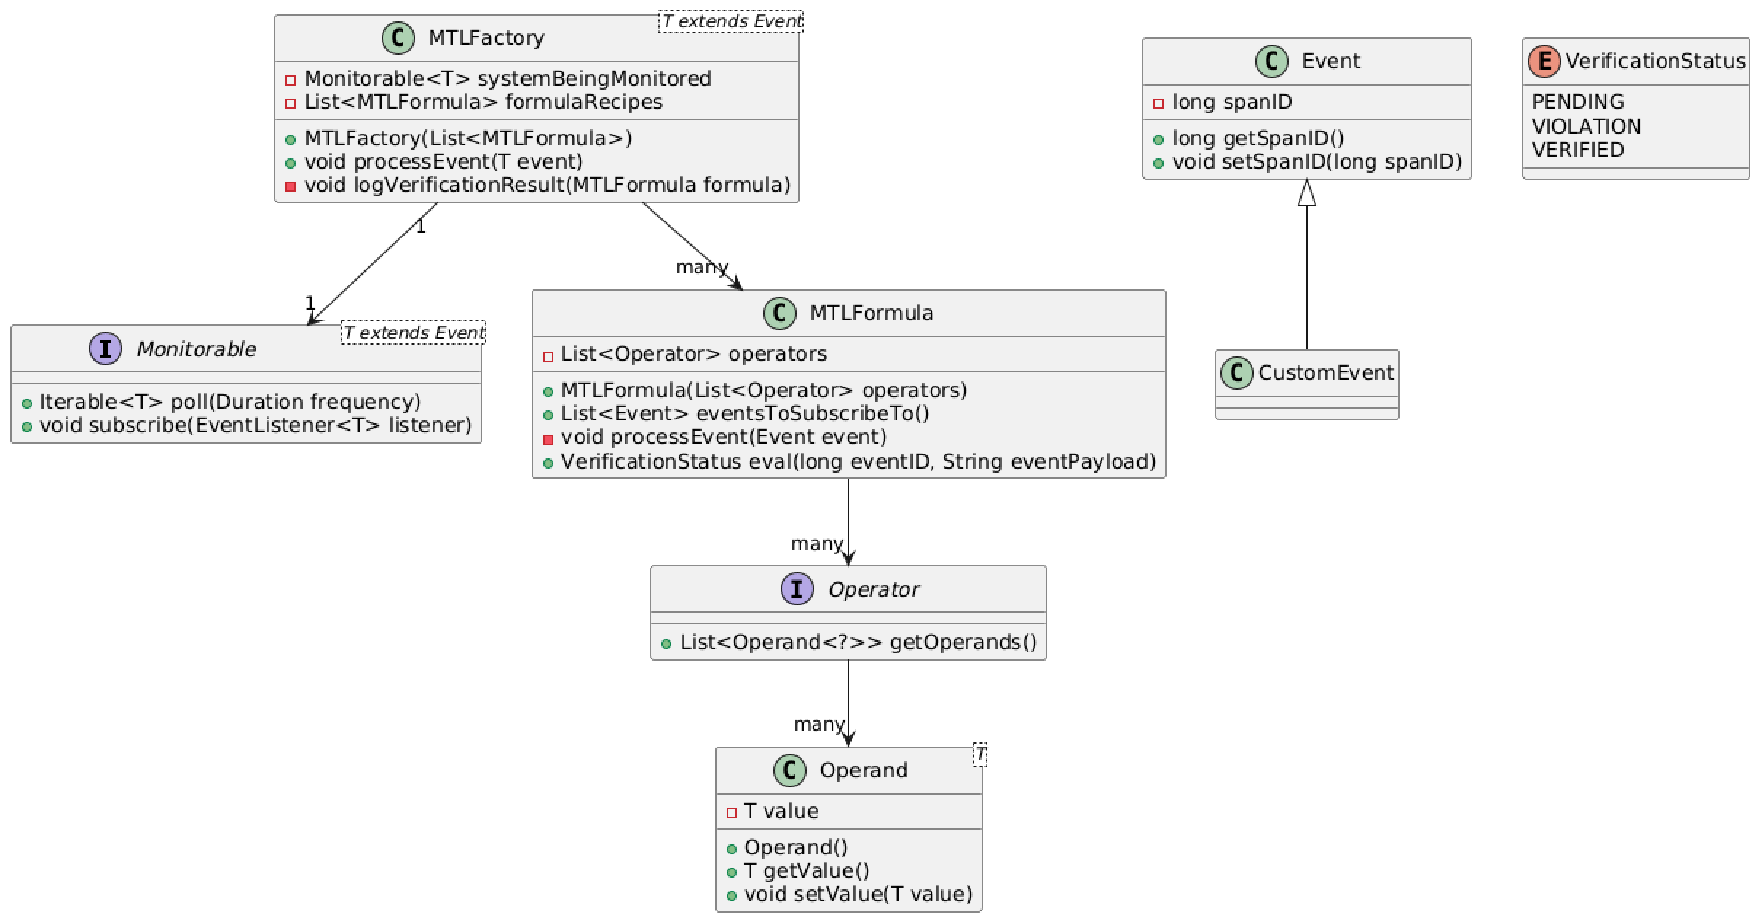
\includegraphics[width=3in]{uml-diagram.pdf}


\section{Case Study: An Integrated E-Commerce System}
We will showcase how this approach would look like in the scenario of an integrated e-commerce system.
The process we are attempting to verify is the fundamental user journey in e-commerce.
It begins with a user that has a full cart and submits the payment information in the website.
The response can either be a successfull payment event or a failed payment event.
Once the payment goes through, the event emitted is consumed by a notification system that sends an email to the user.
In addition, the successfull payment event is consumed by a supply chain software that updates the inventory and emits
a respective inventory update event.
Lastly, the successfull payment event is consumed by the shipment delivery system that adds a new shipment to be done,
emitting the respective new shipment event, which is followed by a shipment scheduled event that notifies the user when
the package ordered will arrive.


Finally, when the user receives the package, the person responsible for its delivery submits a shipment completed event,
and the user journey finishes.
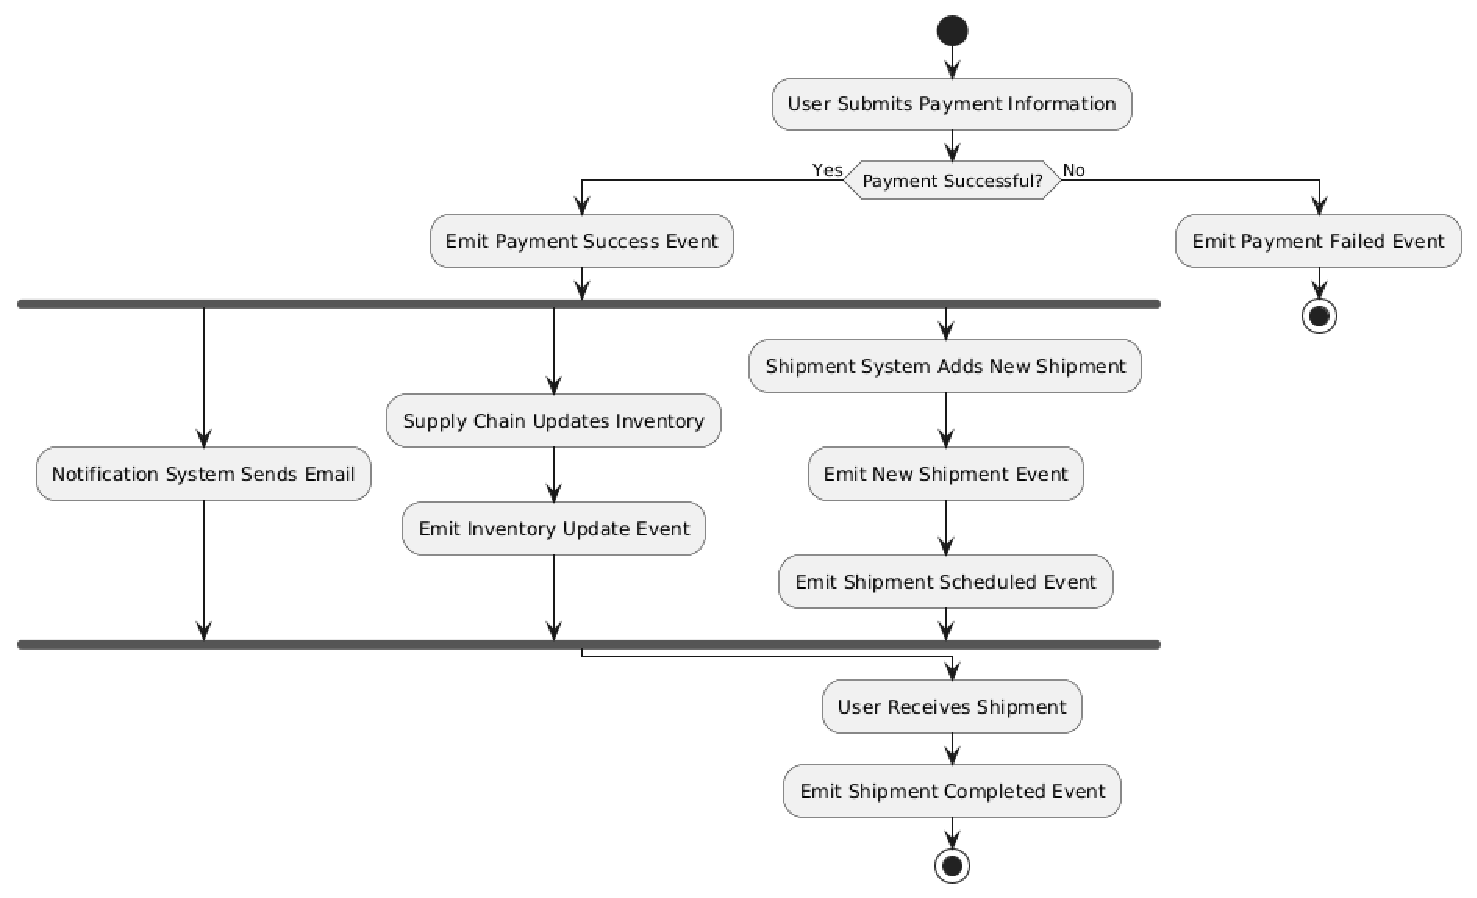
\includegraphics[width=3.2in]{events-diagram.pdf}

A few desirable properties for which we would want to check that they hold and know when they don't due to
system failures are the following:
\begin{enumerate}
	\item After the user paying(proposition CL), a payment completed(proposition PC) or a payment failed(proposition PF) event arrives in X time
	\item A shipment should be scheduled(proposition SCH) within 24 hours of the user having paid.
	\item If the user specified same day delivery, the Shipment Completed(proposition SC) Event should be within 24 hours of the payment completed event.
\end{enumerate}
The properties of the system can be expressed in MTL in the following manner:
\begin{align}
	 & \Box (CL \implies \lozenge_{\leq 5sec}( PC \lor PF)) \\
	 & \Box (PC \implies \lozenge_{\leq 24h} SCH)           \\
	 & \Box (SDD \implies \lozenge_{\leq 24h} SC )
\end{align}


\section{Future Work}
The research presented in this work lays the foundation for practical runtime verification of performance in event-based systems using Metric Temporal Logic (MTL). However, several avenues remain unexplored and present exciting opportunities for future research. Below, we outline key directions for extending this work:

\begin{itemize}
	\item \emph{Rigorous Integration with Application Protocols}: \\
	      A promising direction is the integration of MTL-based runtime verification with widely used application protocols such as \emph{GraphQL}, \emph{gRPC}, and \emph{REST}. These protocols are fundamental to modern distributed systems, and ensuring their compliance with temporal performance properties could significantly enhance system reliability and efficiency. Future work could focus on developing protocol-specific adapters that translate protocol-level events into MTL-compatible formats, enabling seamless verification across diverse communication paradigms.

	\item \emph{Autoscaling Infrastructure Resources in Response to Violations}: \\
	      Another critical area of exploration is the dynamic adjustment of infrastructure resources based on violations of MTL properties. By coupling runtime verification with \emph{autoscaling mechanisms}, systems could proactively respond to performance degradation or violations of temporal constraints. For instance, if an MTL property specifying a maximum response time is violated, the system could automatically scale up computational resources to mitigate the issue. This approach would bridge the gap between runtime verification and adaptive system management.

	\item \emph{Generating Metric Temporal Propositions from Event Logs Using Process Mining}: \\
	      Automating the generation of MTL propositions from event logs using \emph{process mining} techniques represents a significant step toward making runtime verification more accessible. Process mining can uncover patterns and temporal relationships in event logs, which can then be formalized as MTL properties. Future work could focus on developing algorithms and tools to extract meaningful MTL propositions from historical event data, reducing the manual effort required for specification and enabling more comprehensive verification.
\end{itemize}

These future directions aim to expand the applicability and impact of MTL-based runtime verification, making it a more integral part of modern EBS. By addressing these challenges, we can move closer to integrating performance considerations in EBS in a non-invasive manner.



\bibliographystyle{ieeetr}
\bibliography{Research-Methodology-Paper}

\end{document}
